\documentclass[11pt,a4paper]{article}
\usepackage[top=3cm, bottom=3cm, left=2.5cm, right=2.2cm]{geometry} %geometry of page
\usepackage[hidelinks]{hyperref} %reference links
\usepackage{fancyhdr} %header and footer control
\usepackage{minted} %source code syntax highlighting
\usepackage{qrcode} %qrcode links
\usepackage{graphicx} %images
\usepackage{tikz} %diagrams
\usepackage{subcaption} %sub-figures
\usepackage{parskip}
\usetikzlibrary{calc, positioning}
\usepackage{pgfplots} %plots
\usepgfplotslibrary{groupplots}
\pgfplotsset{compat=1.18}

\linespread{1.3}
\emergencystretch 3em

% Set Header and Footer
\fancyhead{}
\fancyhead[L]{\textbf{Control system}}
\fancyhead[R]{max.champneys@sheffield.ac.uk}
\fancyfoot{}
\fancyfoot[L]{\thepage}
\fancyfoot[R]{MAC 233 Arduino Labs, School of MAC, University of Sheffield}

% the routine repeated at every build step in Phase 1
\newcommand{\routine}[1]{%
    \par\noindent\fbox{\parbox{\dimexpr\textwidth-2\fboxsep-2\fboxrule}{#1}}\par
}

% a warning that must not be missed
\newcommand{\warning}[1]{%
    \par\noindent{\setlength{\fboxrule}{1.2pt}\setlength{\fboxsep}{8pt}%
    \fcolorbox{red}{red!6}{\parbox{\dimexpr\textwidth-2\fboxsep-2\fboxrule}{#1}}}\par
}

% Create Document
\begin{document}
\pagestyle{fancy}

\section*{Prerequisites}
This worksheet builds on all four of the lab activities. It reuses the LED circuit from Lab 2, the servo from Lab 3 and the hall effect sensor and interrupt from Lab 4, and none of these will be explained in detail again here. Out of your Arduino pack, you will need: 1 Arduino, 1 breadboard, 2 A3144 hall effect sensors, 1 magnet, 4 LEDs, 4 $220\Omega$ resistors, 2 $10K\Omega$ resistors, 1 servo, and jumper cables. For the final build step you will also need your mini rig, the motor driver and a 9V battery.

\section*{Objectives}
Over the next three weeks, we will build a working control system for the mini-rig e-bikes that you have manufactured this semester: an Arduino that reads how fast the rider is pedalling and how fast the wheel is turning, and decides how much help the motor should give. By the end, you will have everything you need to design and test your own control system next semester.

Along the way, you will learn and practise a methodical approach: building a system up one piece at a time, and checking that each piece works before adding the next. This way of thinking is critical when we are working with both hardware and software!

\section*{The plan}
Getting electronics, code and hardware to all work together at once is never an easy task in engineering!\footnote{Or `integration hell' as it is sometimes called.} Whilst we could build up all the electronics, then write the code and connect the rigs straight away, if we have problems it might be hard to tell where they are coming from.

Instead, we will take a methodical approach. First we will cover how the control system will work and go through a sketch together. Then, we will add each component in turn and test it to make sure that it is working correctly. Once we are happy that the hardware and software are working as expected, we will think about how we can modify the control system to be more effective. Table \ref{tab:plan} shows roughly where you should be each week, although this is ultimately up to you!

\begin{table}[ht]
    \centering
    \begin{tabular}{lll}
        \textbf{Week} & \textbf{Phase} & \textbf{Do you need your mini rig?} \\
        \hline
        7 & Phase 0: how the control system works & No \\
          & Phase 1: build steps 1--3 & No, test the sensors with a magnet \\
        8 & Phase 1: build steps 4--5 & Only for step 5 \\
        9 & Phase 2: developing the control system & Yes \\
    \end{tabular}
    \caption{The plan for weeks 7 to 9.}
    \label{tab:plan}
\end{table}

Don't worry if your mini rig isn't finished at the start of week 8. Build steps 1 to 4 only need your Arduino, your breadboard and a magnet: wherever a step asks you to turn the crank or the wheel, you can pass the magnet past the sensor by hand instead. When your rig is ready, `Moving onto your mini rig' (page \pageref{sec:rig}) explains how to move your sensors onto it.

% number the sections from 0 so that they match the phases
\setcounter{section}{-1}
\section{Phase 0: how the control system works}
\label{sec:phase-0}

\subsection{The big picture}
An e-bike motor shouldn't run all the time. In the UK, an electrically assisted pedal cycle may only help the rider while they are pedalling, and must stop helping once the bike reaches 25\,km/h. Our control system therefore needs to know two things: how fast the rider is pedalling, and how fast the bike is going. It gets these from two hall effect sensors, one watching a magnet on the crank and one watching a magnet on the wheel (Figure \ref{fig:mini-rig}), exactly as in Lab 4.

\begin{figure}[ht]
    \centering
    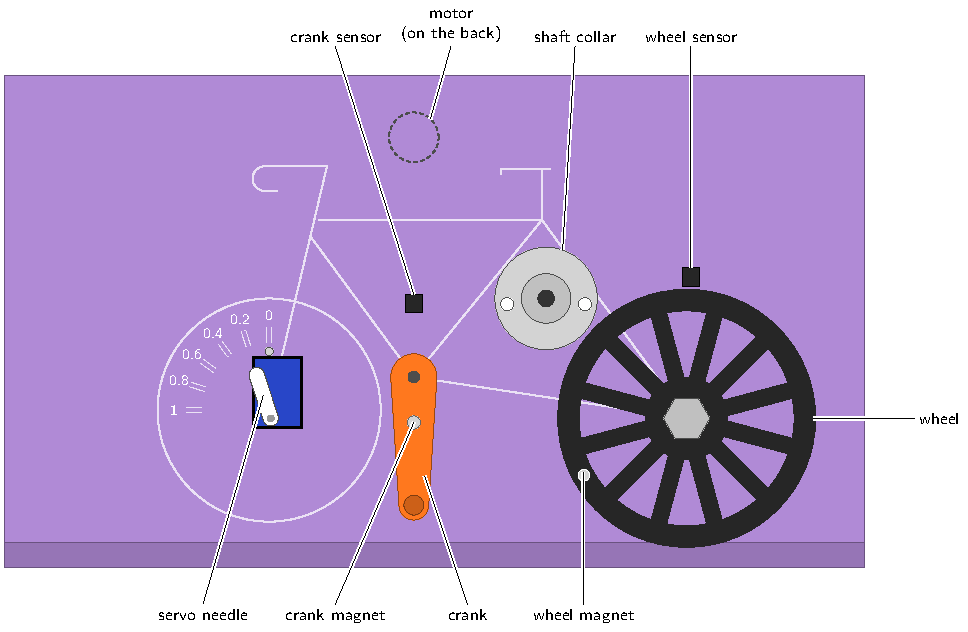
\includegraphics[width=\textwidth]{../images/mini-rig.pdf}
    \caption{The mini rig, seen from the front. The motor is mounted on the back of the panel.}
    \label{fig:mini-rig}
\end{figure}

From these two measurements, the Arduino decides on a \textit{motor demand}: a number between 0 (motor off) and 1 (full power). On the mini rig, this demand drives the motor through a motor driver, and is also shown by a servo acting as a needle (Figure \ref{fig:big-picture}).

There are also four LEDs, which we will use to check each part as we build it. The ready LED comes on once the sketch has started up. The crank and wheel LEDs flash each time their sensor sees the magnet, and the motor LED is on whenever the sketch wants the motor to help. These LEDs will help us ensure each part of our control system is working as intended. 

\begin{figure}[ht]
    \begin{center}
        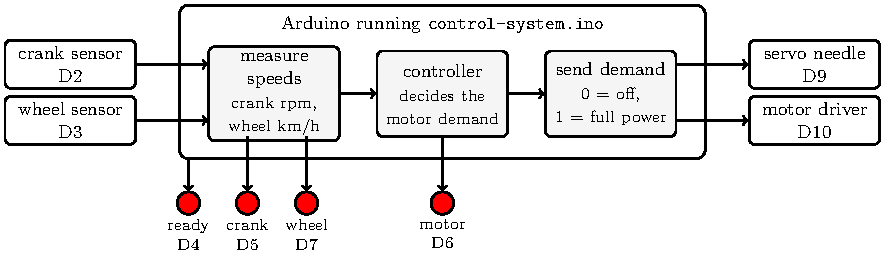
\includegraphics{../images/block-diagram.pdf}
    \end{center}
    \caption{The control system, with the Arduino pin for each part. The LEDs hang off the part of the sketch that switches them.}
    \label{fig:big-picture}
\end{figure}

\subsection{The sketch}
Unlike the previous labs, this sketch will be provided as-is, and you won't change anything in it until Phase 2. Download \verb|control-system.ino| from \url{https://github.com/MDCHAMP/MAC233/blob/main/control-system/control-system.ino} and open it in Arduino IDE. This section walks through what each part does and concludes with a check of your understanding.

\subsubsection{The parts you must not change}
The top of the sketch is fenced off with a \verb|DO NOT CHANGE THESE VALUES| box. The first part names the pins. These match the wiring of the big rigs, so they are fixed:
\inputminted[
    autogobble, stripnl, breaklines,
    rangeregex={(?ms)^.define SYSTEM_READY_LED_PIN.*?ESC_PIN 9 *//},
]{arduino}{../control-system.ino}
\vspace{.75em}

The second part holds the safety limits. The two \verb|ACTIVITY_DELAY| values are the 500-millisecond LED windows from Lab 4. The two \verb|MAXIMUM_DELAY| values say that if a sensor hasn't seen its magnet for 3 seconds, that part of the bike is treated as stopped. \verb|WHEEL_MAXIMUM_SPEED| is the 25\,km/h assist limit, and \verb|WHEEL_CIRCUMFERENCE| is the distance a real bike wheel travels in one turn, in metres:
\inputminted[
    autogobble, stripnl, breaklines,
    rangeregex={(?ms)^.define CRANK_PASS_ACTIVITY_DELAY.*?pedal_threshold_rpm = 20; *//},
]{arduino}{../control-system.ino}
\vspace{.75em}

\subsubsection{Setup function}
Most of the `setup' function is familiar from the labs: it starts the serial connection, sets the four LED pins to outputs and turns them off, and attaches the servo. The interesting part is at the end:
\inputminted[
    autogobble, stripnl, breaklines,
    rangeregex={(?ms)^ *// pause system until ready.*?Serial.println\\("System Ready"\\);},
]{arduino}{../control-system.ino}
\vspace{.75em}

Notice that the sensors' interrupts are only attached \textit{after} the 3-second pause. Anything the sensors see while the system is starting up is never recorded, so the motor can't be switched on by something that happened while the system wasn't ready. Only then does the ready LED come on.

\textit{Note:} the sensor pins use \verb|INPUT_PULLUP| rather than the \verb|INPUT| from Lab 4. This turns on a resistor inside the Arduino that holds the pin \verb|HIGH| when nothing is connected to it. Without it, a pin with no sensor attached yet `floats' between high and low, and can trigger the interrupt at random. 

\subsubsection{Interrupts: counting passes of the magnet}
Each sensor has its own interrupt function. Every time the magnet passes, it adds one to a counter and remembers the times of this pass and the one before:
\inputminted[
    autogobble, stripnl, breaklines,
    rangeregex={(?ms)^void crankInterrupt.*?^\\x7d},
]{arduino}{../control-system.ino}
\vspace{.75em}

The wheel's interrupt, \verb|wheelInterrupt|, does the same, with one extra check: a second pass within 200 milliseconds of the last one is ignored, in case the sensor `bounces' and reports a single pass twice.

\subsubsection{Loop function: from passes to speeds}
At the start of every loop, the sketch turns the crank and wheel LEDs on if their sensor has seen the magnet in the last 500 milliseconds, just as in Lab 4. It then works out how fast the crank is turning. The time between the last two passes is the time for one turn, so dividing 60 seconds by it gives the speed in revolutions per minute (rpm):
\inputminted[
    autogobble, stripnl, breaklines,
    rangeregex={(?ms)^ *float crank_rpm = 0;.*?^ +\\x7d},
]{arduino}{../control-system.ino}
\vspace{.75em}

The \verb|if| statement only calculates a speed if the sensor has been passed at least twice (one pass on its own can't tell us how long a turn took), and if the last pass was less than 3 seconds ago. Otherwise, the speed stays at zero.

The wheel speed is worked out the same way, then converted to km/h: the wheel's rpm, times 60 minutes, times the circumference of the wheel, gives metres per hour, and dividing by 1000 gives km/h.

\subsubsection{The example controller}
The middle of the `loop' function, between the two lines of slashes, is where your control system goes. To start with, it holds a simple example:
\inputminted[
    autogobble, stripnl, breaklines,
    rangeregex={(?ms)^ *const float motor_step_up.*?motor_demand\\(motor_power\\); // send that power to the motor},
]{arduino}{../control-system.ino}
\vspace{.75em}

While the rider is pedalling (the crank is turning faster than 20\,rpm) and the bike is below 25\,km/h, the motor LED comes on and \verb|motor_power| creeps up by 0.008 every loop. Otherwise, the LED goes off and \verb|motor_power| creeps down by 0.01 every loop. \verb|constrain| keeps it between 0 and 1. Because the change is small each time, the motor speeds up and slows down smoothly over a few seconds, rather than jumping straight between off and full power.

\subsubsection{Sending the demand to the motor}
Finally, \verb|motor_demand| sends the demand out in two forms: as a servo signal on pin D9 (the motor controller on the big rig, and the needle on the mini rig), and as a PWM signal on pin D10, which drives the motor driver on the mini rig:
\inputminted[
    autogobble, stripnl, breaklines,
    rangestartstring={void motor_demand(float demand)},
]{arduino}{../control-system.ino}
\vspace{.75em}

Every second, the `loop' function also prints a status message to the serial monitor, like this one:
\begin{minted}{text}
motor demand: 0.00 crank count: 0 wheel count: 0 crank rpm: 0.00 wheel kmph: 0.00
\end{minted}
\vspace{.75em}

\subsection{Check your understanding}
Before you build anything, try to answer these with a partner. You will need the answers in Phase 1.
\begin{enumerate}
    \item The magnet has passed the crank sensor exactly once. What will \verb|crank_rpm| be, and why?
    \item The magnet passes the crank sensor once every 1.5 seconds. What is \verb|crank_rpm|? Will the example controller turn the motor on?
    \item The rider stops pedalling. Roughly how long is it before the motor LED goes out?
    \item \verb|motor_power| is 1 when the rider stops pedalling. The `loop' function runs about 35 times a second. Roughly how long does the motor take to stop?
    \item The magnet passes the wheel sensor once a second. Roughly what speed, in km/h, will the serial monitor show?
\end{enumerate}

\section{Phase 1: building and verifying the electronics}
\label{sec:phase-1}
We will now build the electronics in five steps, adding one or two components each time. Upload \verb|control-system.ino| to your Arduino once, at the start of step 1, and then leave it alone: the code stays the same while the hardware grows. At every step, follow the same routine:

\routine{%
    \textbf{Build}: add only the new components shown in full colour in the figure. Parts from earlier steps are shown faded.\\
    \textbf{Predict}: before you power anything up, write down what you expect the LEDs and the serial monitor to do. Don't read ahead!\\
    \textbf{Test}: try it, and compare what happens with your prediction.\\
    \textbf{If not\ldots}: if something doesn't match, stop and fix it before moving on. Because only one thing has changed since the last step worked, the fault is almost certainly in what you just added.
}

The figures show one way of laying out the breadboard. Use them as a guide: you can put components in any rows you like, as long as the connections are the same. All the figures use the same colours: red wires carry +5V, black wires are GND, and yellow wires carry signals. The servo and the motor driver keep the colours of their own cables. For every LED, the long leg goes towards the resistor and the short leg into the GND rail.

\subsection{Step 1: power and the system ready LED}
\begin{figure}[ht!]
    \begin{center}
        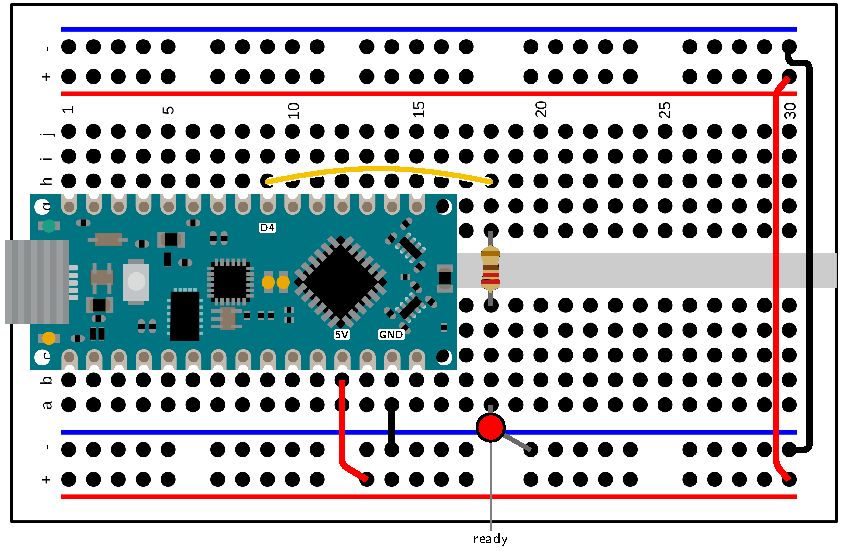
\includegraphics[width=.8\textwidth]{../images/wiring-step-1.pdf}
    \end{center}
    \caption{Step 1: power to the rails, and the system ready LED on D4.}
    \label{fig:step-1}
\end{figure}

\textbf{Build} (Figure \ref{fig:step-1}): place the Arduino across the centre channel of the breadboard. Connect its GND and +5V pins to the $-$ and $+$ rails, and link the rails on both sides of the board so that every rail is powered. Then wire the ready LED as in Lab 2: Arduino D4\textrightarrow $220\Omega$ resistor\textrightarrow LED\textrightarrow GND.

\textbf{Predict}: connect the USB cable and upload \verb|control-system.ino|. What should the ready LED do, and when? What should the serial monitor show?

\textbf{Test}: open the serial monitor (9600 baud) and press the reset button on the Arduino. About 3 seconds after reset, the ready LED should come on and stay on, and \verb|System Ready| should appear, followed by a status message every second with every value at zero.

\textbf{If not\ldots}: does the serial monitor show anything at all? If it does, but the LED stays off, is the LED the right way round, and is it in the same row as its resistor?

\subsection{Step 2: the crank sensor and crank LED}
\begin{figure}[ht!]
    \begin{center}
        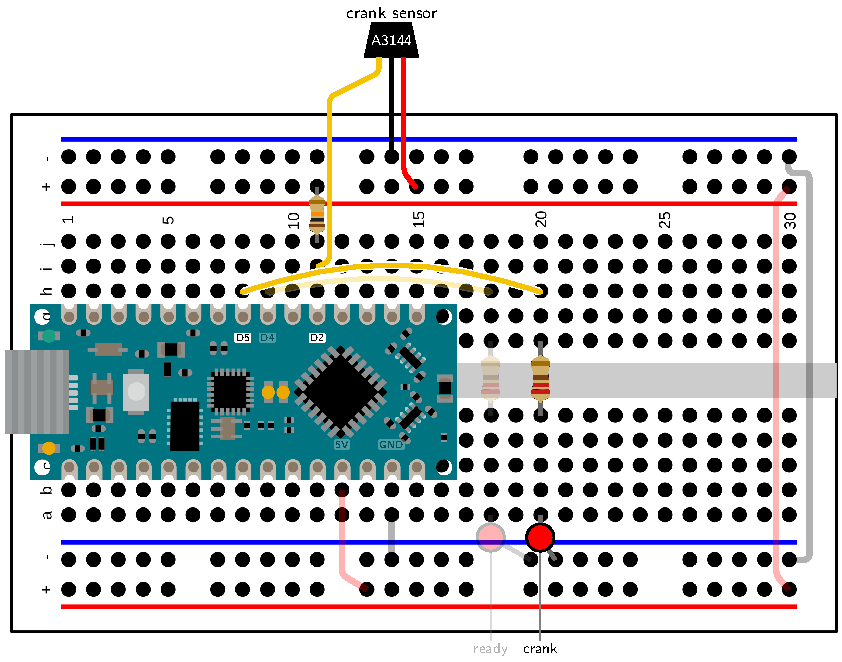
\includegraphics[width=.8\textwidth]{../images/wiring-step-2.pdf}
    \end{center}
    \caption{Step 2: the crank sensor on D2, and the crank LED on D5.}
    \label{fig:step-2}
\end{figure}

\textbf{Build} (Figure \ref{fig:step-2}): wire the crank sensor as in Lab 4: sensor +5V leg\textrightarrow +5V, sensor GND leg\textrightarrow GND, sensor output\textrightarrow Arduino D2, with a $10K\Omega$ resistor between D2 and +5V. The sensors are drawn on leads, as they will be on your rig; until then, connect your sensor's legs to the board with jumper cables. Then wire the crank LED in the same way as the ready LED: Arduino D5\textrightarrow $220\Omega$ resistor\textrightarrow LED\textrightarrow GND.

\textbf{Predict}: what will the crank LED do when you pass the magnet past the sensor once? What will \verb|crank count| and \verb|crank rpm| show after one pass? After two passes, a second apart? And what do you think will happen to \verb|motor demand| if you keep passing the magnet about once a second, even though there is no motor connected yet?

\textbf{Test}: pass the magnet slowly past the crank sensor. Every pass should light the crank LED for half a second and add one to \verb|crank count|. \verb|crank rpm| should stay at zero after the first pass, then show about 60 if you pass the magnet again a second later, and fall back to zero 3 seconds after you stop. \verb|wheel count| should stay at zero throughout. If you keep passing the magnet, \verb|motor demand| should climb towards 1, then fall back to zero once you stop. The sketch is already doing its job, even though there is nothing for it to control yet.

\textbf{If not\ldots}: does \verb|crank count| go up, even though the LED stays off? Then the sensor is working, and the problem is in the LED circuit. If neither changes, try turning the magnet over: the sensor only responds to one pole.

\subsection{Step 3: the wheel sensor and wheel LED}
\begin{figure}[ht!]
    \begin{center}
        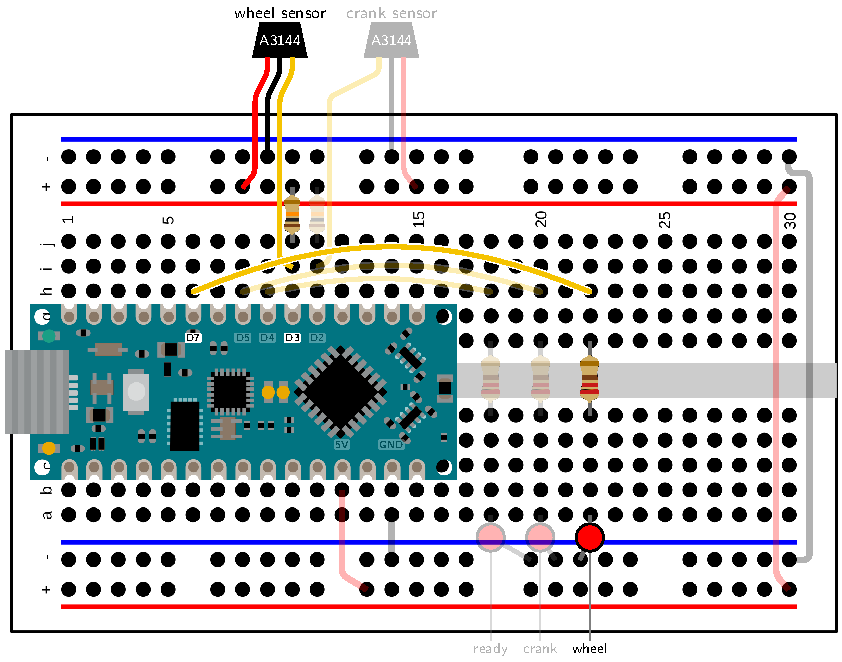
\includegraphics[width=.8\textwidth]{../images/wiring-step-3.pdf}
    \end{center}
    \caption{Step 3: the wheel sensor on D3, and the wheel LED on D7.}
    \label{fig:step-3}
\end{figure}

\textbf{Build} (Figure \ref{fig:step-3}): wire the wheel sensor exactly as you did the crank sensor, but with its output to Arduino D3 and its own $10K\Omega$ resistor between D3 and +5V. Then wire the wheel LED: Arduino D7\textrightarrow $220\Omega$ resistor\textrightarrow LED\textrightarrow GND.

\textbf{Predict}: which values on the serial monitor should change when you pass the magnet past the wheel sensor, and which shouldn't? Using your answer to question 5 in Phase 0, what should \verb|wheel kmph| show if you pass the magnet once a second?

\textbf{Test}: each pass should light the wheel LED and add one to \verb|wheel count|, while the crank values stay where they were. One pass a second should give a \verb|wheel kmph| of about 7.5. Then repeat the step 2 test on the crank sensor, to check that it still works.

\textbf{If not\ldots}: does passing the magnet past the wheel sensor change the \textit{crank} values? Check which pin each sensor's output is connected to.

\subsection{Step 4: the motor LED and the servo}
\begin{figure}[ht!]
    \begin{center}
        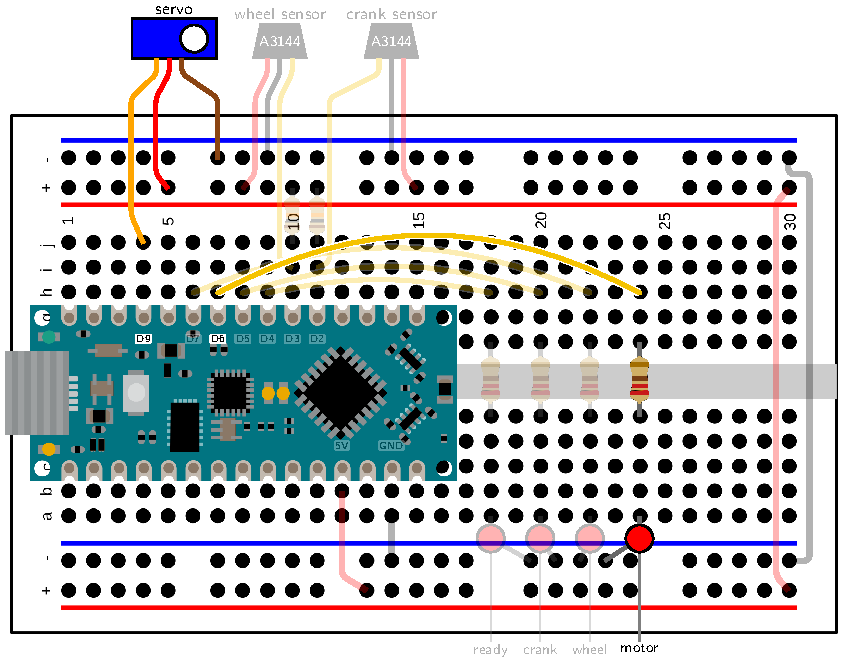
\includegraphics[width=.8\textwidth]{../images/wiring-step-4.pdf}
    \end{center}
    \caption{Step 4: the motor LED on D6, and the servo on D9.}
    \label{fig:step-4}
\end{figure}

\textbf{Build} (Figure \ref{fig:step-4}): wire the motor LED: Arduino D6\textrightarrow $220\Omega$ resistor\textrightarrow LED\textrightarrow GND. Then connect the servo as in Lab 3: signal (orange)\textrightarrow Arduino D9, power (red)\textrightarrow +5V, ground (brown)\textrightarrow GND.

\textbf{Predict}: you pass the magnet past the crank sensor once a second for 10 seconds, then stop. Describe what the motor LED and the servo needle will do, and when. What if you pass the magnet only once every 4 seconds instead?

\textbf{Test}: pedalling, simulated by passing the magnet past the crank sensor about once a second, should turn the motor LED on from the second pass, while the servo needle sweeps up steadily over 3 to 4 seconds. When you stop, the LED should stay on for up to 3 more seconds, and then go off while the needle sweeps back down. Passing the magnet once every 4 seconds should never turn the motor LED on.

\textbf{If not\ldots}: does \verb|motor demand| on the serial monitor rise and fall as expected? If it does, the controller is working and the problem is in the circuit you just added.

% unnumbered, so that each build step's number matches its subsection
\subsection*{Moving onto your mini rig}
\label{sec:rig}
Once your mini rig is ready, fix the crank and wheel sensors to it so that their magnets pass close by once per turn. The wiring on the breadboard doesn't change. Then repeat the tests from steps 2 to 4, turning the crank and the wheel slowly by hand instead of moving the magnet. Every turn should give exactly one blink of the right LED.

\subsection{Step 5: the motor driver (requires mini rig)}
\begin{figure}[ht!]
    \begin{center}
        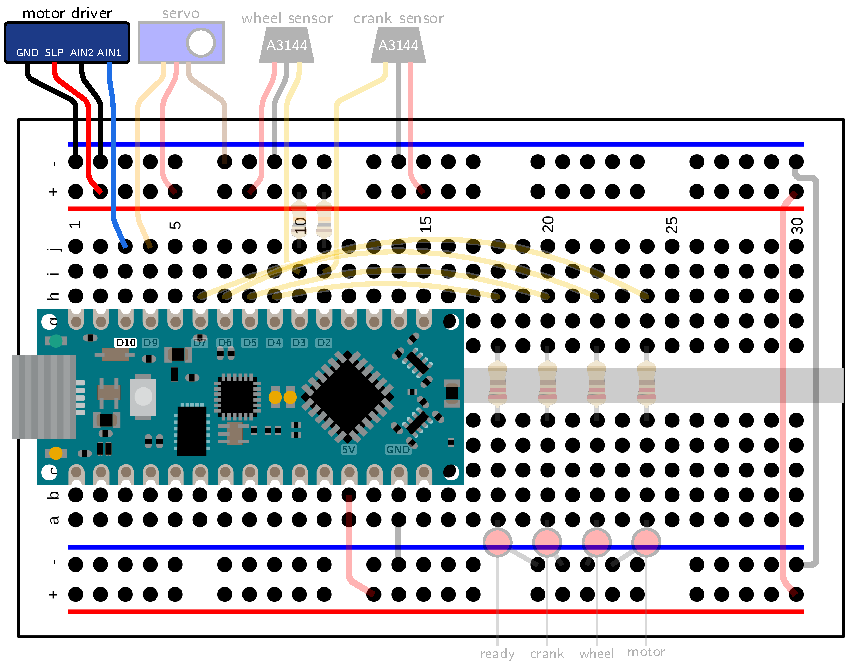
\includegraphics[width=.8\textwidth]{../images/wiring-step-5.pdf}
    \end{center}
    \caption{Step 5: the motor driver, controlled by D10.}
    \label{fig:step-5}
\end{figure}

The Arduino can't power the motor itself: its pins can only supply a tiny current, far less than a motor needs, and a motor can send voltage spikes back that would damage the Arduino. A motor driver sits between the two. It takes its power from a separate supply that is big enough for the motor, and uses the small signal from the Arduino to decide how much of that power to pass on. For this external power supply, we will be using a 9V battery. 

\warning{%
    \textbf{\textcolor{red}{Warning: 9V will destroy your Arduino.}} The 9V battery only ever clips onto the battery snap soldered to the motor driver. Never connect it to the breadboard: the Arduino runs on 5V, and 9V on the +5V rail will damage it permanently. While the battery is connected, don't let the motor driver's pins touch the Arduino or the breadboard either: some of them carry the battery's 9V. Ask a GTA to check your wiring before you clip the battery on for the first time.
}

The Arduino tells the driver how hard to run the motor with a PWM signal on D10, set from the motor demand: the higher the demand, the more power the motor gets. Figure \ref{fig:motor-driver} shows the driver board and the connections we use.

\begin{figure}[ht!]
    \begin{center}
        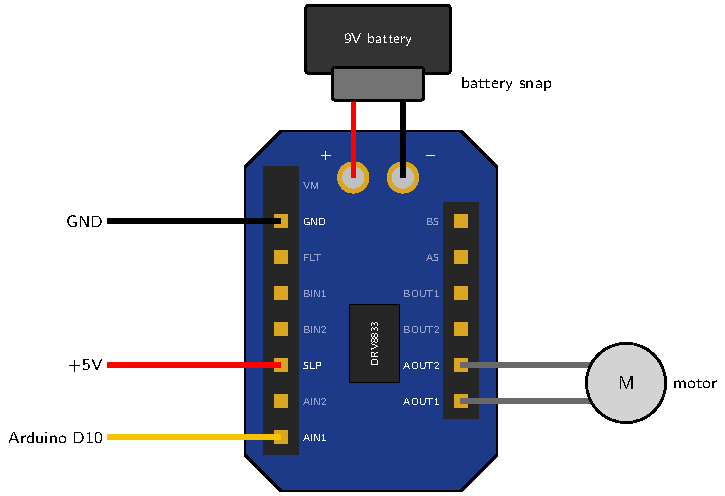
\includegraphics[width=.6\textwidth]{../images/motor-driver.pdf}
    \end{center}
    \caption{The motor driver board, seen from above. Only the pins with bright labels are used: four come from the breadboard, the 9V battery clips onto the battery snap soldered to the top of the board, and the motor connects to the two outputs on the right.}
    \label{fig:motor-driver}
\end{figure}


\textbf{Build} (Figure \ref{fig:step-5}): connect the motor driver: AIN1 (blue)\textrightarrow Arduino D10, SLP (red)\textrightarrow +5V, GND (black)\textrightarrow GND, AIN2 (black)\textrightarrow GND. Note that the driver has two black wires, and both go to GND. The motor itself and its power supply connect to the driver, not to the breadboard.

\textbf{Predict}: you turn the crank steadily by hand. What will the wheel do, and how will it compare with the servo needle?

\textbf{Test}: turning the crank steadily should make the motor start to drive the wheel, speeding up smoothly as the needle rises. When you stop turning the crank, the motor should slow down and stop as the needle falls.

\textbf{If not\ldots}: does the needle still move as it did in step 4? If it does, the Arduino is sending the right demand, and the problem is between D10 and the motor.

\section{Phase 2: developing the control system}
\label{sec:phase-2}
With every part built and checked, we can now ask how good the example controller actually is, and how you might improve it.

\subsection{Testing the example controller}
Turn the crank steadily by hand, at roughly one turn a second, for about 20 seconds, then stop. While you do, watch the servo needle, the wheel and the serial monitor. Afterwards, copy the status messages out of the serial monitor so you can look at how \verb|motor demand| and \verb|wheel kmph| changed over time. Before you start, sketch what you think the two will look like.

\subsection{What we want vs what we get}
Figure \ref{fig:want-vs-get} compares what we would like the system to do with what the example controller typically does on a mini rig. Ideally, the motor would give full help for as long as the rider is pedalling, so that the bike speeds up quickly and rides right up to the 25\,km/h limit, and it would stop helping as soon as the rider stops. What we get is different in three ways.

\begin{figure}[ht!]
    \begin{center}
        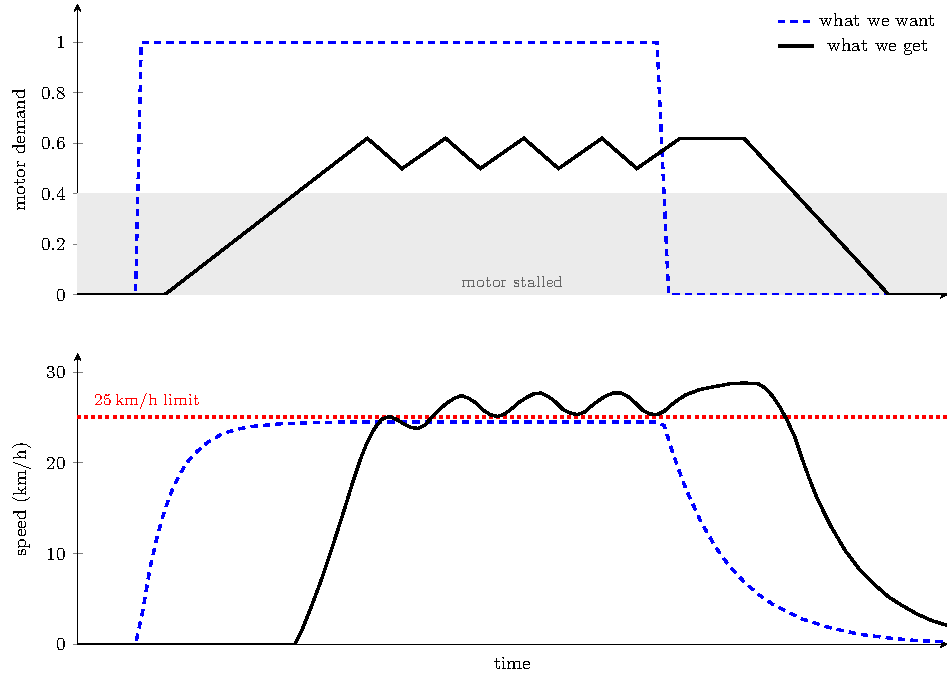
\includegraphics[width=\textwidth]{../images/want-vs-get.pdf}
    \end{center}
    \caption{What we want (dashed) and what we typically get (solid) for the motor demand (top) and the bike's speed (bottom), while the rider pedals and then stops. The curves are illustrative: the exact numbers vary a lot from rig to rig.}
    \label{fig:want-vs-get}
\end{figure}

\textbf{A slow, delayed start.} The demand ramps up from zero, but the motor doesn't turn at all until the demand reaches roughly 0.4. Below that, the motor's power isn't enough to overcome friction in the motor, the gears and the wheel, so the motor is \textit{stalled}. Almost half of the ramp is spent getting nowhere.

\textbf{Overshoot and wobble around the limit.} The controller only knows two things: keep increasing the demand, or decrease it. The bike goes past 25\,km/h before the controller notices, because the wheel speed is only measured once per turn, and the wheel's inertia keeps it going for a moment after the demand starts to fall. The speed then drops below the limit, the controller ramps up again, and the cycle repeats.

\textbf{Help that carries on after the rider stops.} The crank speed is only reset to zero 3 seconds after the last pass of the magnet, so the motor keeps helping for up to 3 seconds after the rider stops, and only then ramps down.

\subsection{Improving the controller}
Now it's your turn. Everything between the two lines of slashes in the `loop' function is yours to change, but leave the \verb|DO NOT CHANGE THESE VALUES| block alone. Some ideas to start from:
\begin{itemize}
    \item Start the ramp from just below the point where your motor starts to turn, rather than from zero.
    \item Instead of only increasing or decreasing the demand, set it from how far the bike is below the speed limit, so that the motor eases off as the bike approaches 25\,km/h.
    \item Change the ramp rates, and see how they affect the overshoot.
\end{itemize}

Use the same methodical approach as in Phase 1: change one thing at a time, predict what it will do, then test it and compare.

\pagebreak
\section*{Help}
If you have lost track of the sketch or want to check you have the latest version, you can find it at \url{https://github.com/MDCHAMP/MAC233/blob/main/control-system/control-system.ino}.

\begin{center}
    \qrcode[hyperlink, height=4cm]{https://github.com/MDCHAMP/MAC233/blob/main/control-system/control-system.ino}
\end{center}

\vspace{2em}

The completed breadboard, with every component from steps 1 to 5, is below.

\begin{center}
    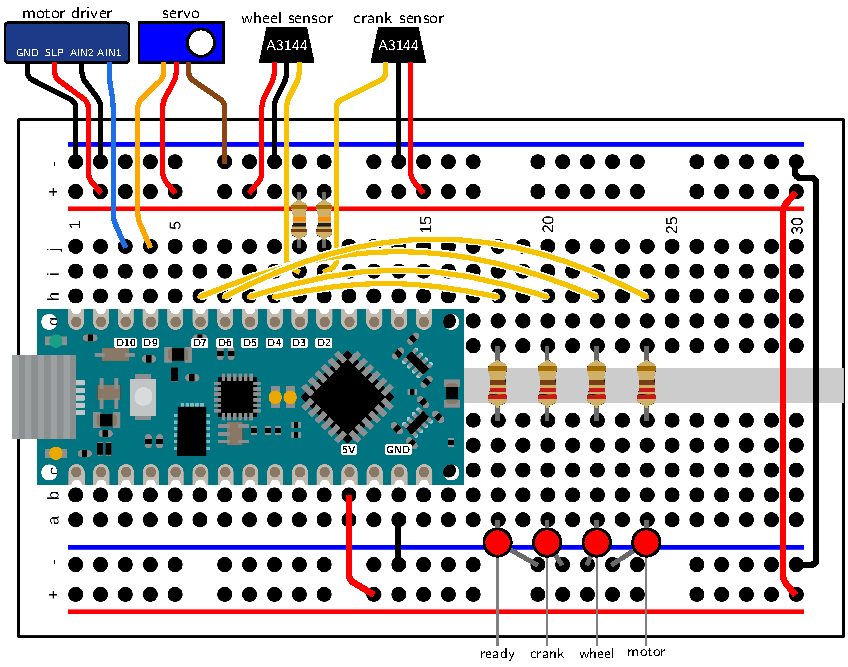
\includegraphics[width=.8\textwidth]{../images/wiring-complete.pdf}
\end{center}

\end{document}
